\documentclass[11pt]{article}

\usepackage{amsmath, amssymb, amsthm}
\usepackage{graphicx}
\usepackage{booktabs}
\usepackage{hyperref}
\usepackage{geometry}
\usepackage{xcolor}
\usepackage{caption}

\geometry{margin=1in}
\hypersetup{
  colorlinks=true,
  linkcolor=blue,
  urlcolor=blue,
  citecolor=blue
}

\title{Do Neural Networks Learn Structure-Preserving Maps?\\
       A Case Study in Latent-to-Hilbert Embeddings}

\author{Adnan \\
        \texttt{https://github.com/adnanphp/diffusion-hilbert}}

\date{\today}

\begin{document}
\maketitle

\begin{abstract}
We investigate whether neural networks can learn structure-preserving
mappings from a compressed latent space to a Hilbert-space representation,
such that inner products between latent points correspond to inner products
between target points. Using a controlled setup---an 8-dimensional
autoencoder bottleneck on MNIST, $n$-qubit product-state targets constructed
via PCA-based angle encoding, and small MLPs trained with a combined
mean-squared-error (MSE) and inner-product loss---we report four findings.
First, the mapping is approximately linear, with a linear regression from
the latent to the recovered angle space achieving $R^{2} = 0.91$; the
learned map's primary direction is target-driven rather than input-driven,
with cosine similarity $0.989$ to the target's principal direction and
$0.002$ to the input's principal direction. Second, the learned map is
genuinely rank-4: removing any singular direction degrades inner-product
preservation by a factor of $2.5$--$5.9$, despite a singular-value spectrum
with two dominant and two small values. Third, the learned subspace does
not coincide with the PCA basis used to construct the target; different
random seeds recover the same primary direction but diverge in higher-rank
structure. Fourth, in this controlled setting, kernel ridge regression with
an RBF kernel can outperform a tuned MLP (IP error $0.0144$ vs.\ $0.0197$
after 24-configuration tuning), suggesting that for approximately linear
structure-preserving mappings, classical kernel methods may be a simpler
and more effective alternative. We discuss implications for representation
alignment and for the design of structure-preserving neural architectures.
\end{abstract}

\section{Introduction}

Machine learning has increasingly focused on learning \emph{representations}
rather than direct input--output mappings. A recurring problem in this
context is measuring whether two learned representations preserve the same
underlying structure. Canonical correlation analysis \cite{raghu2017svcca},
centered kernel alignment \cite{kornblith2019similarity}, and
Procrustes-based alignment \cite{gower1975generalized} are widely used to
compare representations, but they typically assume a fixed target and ask
whether a learned representation is close to it. In this paper, we ask a
related but distinct question: given a latent vector $z$ and a target
Hilbert-space representation $\psi$, can a neural network learn a mapping
$f(z) = \psi$ that preserves inner products between points?

This question has practical relevance in settings where geometric structure
matters---representation alignment, structure-preserving embeddings, and
classical-to-quantum mappings---and is theoretically motivated by the
desire to understand when a neural network can recover geometric content
rather than merely fit observations.

We investigate the question in a controlled setting. We use an
8-dimensional autoencoder bottleneck trained on MNIST, and construct a
target Hilbert-space representation via PCA-based angle encoding of the
latent vectors. We train several models---linear regression, an MLP trained
on MSE only, an MLP trained on MSE plus an inner-product loss, and kernel
ridge regression---to map $z$ to $\psi$. We evaluate them on inner-product
preservation error (IP\_err), reconstruction error (MSE), and pairwise
distance preservation error (dist\_err).

Our findings are as follows. First, the learned mapping is approximately
linear, with a linear regression from $z$ to the recovered angle space
achieving $R^{2} = 0.91$, and its primary direction is target-driven rather
than input-driven. Second, the learned map requires all singular directions:
rank reduction degrades IP\_err by a factor of $2.5$ to $5.9$. Third, the
learned subspace does not equal the PCA basis, and seed-to-seed variation
appears in the higher-rank structure while the primary direction remains
stable. Fourth, in this controlled setting, kernel ridge regression with an
RBF kernel outperforms the tuned MLP, suggesting that classical kernel
methods may be preferable when the underlying mapping is approximately
linear.

The remainder of the paper is organized as follows. Section~\ref{sec:related}
reviews related work on representation alignment and kernel methods.
Section~\ref{sec:method} describes the experimental setup. Section~\ref{sec:experiments}
presents results. Section~\ref{sec:discussion} discusses interpretation and
implications. Section~\ref{sec:limitations} outlines limitations and future
work.

\section{Related Work}
\label{sec:related}

\paragraph{Representation similarity.} Comparing two learned representations
has become a standard tool in deep learning analysis. Canonical correlation
analysis (CCA) and its deep variants \cite{raghu2017svcca} compare
representations by finding linear transformations that maximize correlation
between projected views. Centered kernel alignment (CKA)
\cite{kornblith2019similarity} provides an alternative based on Hilbert--Schmidt
independence, invariant to orthogonal transformations and isotropic scaling.
Procrustes analysis \cite{gower1975generalized} finds the orthogonal
transformation that best aligns two point sets, and has been adapted to
compare neural representations under the name orthogonal Procrustes.

These methods all assume a fixed target representation and ask whether a
learned representation is close to it. Our setup is different: we do not
assume that a target representation exists, but rather ask whether a
network can learn a mapping \emph{into} a specified target space while
preserving geometric structure.

\paragraph{Kernel methods.} Kernel ridge regression (KRR)
\cite{saunders1998ridge} is a classic method for nonlinear regression that
combines a linear model in a high-dimensional feature space with $L_{2}$
regularization. With an RBF kernel, KRR can approximate a wide class of
smooth functions and typically serves as a strong baseline for
low-dimensional regression tasks. Our experiments show that KRR outperforms
a tuned MLP in our setting, which is consistent with the fact that our
target mapping is approximately linear.

\paragraph{Quantum machine learning.} Quantum feature spaces have been
proposed as a route to enhanced expressivity in machine learning
\cite{havlicek2019supervised, schuld2021machine}. A common construction maps
classical data to quantum states via angle encoding, and one then applies a
variational quantum circuit before measurement. Our angle encoding follows
this approach; we do not simulate the variational part, but rather use the
resulting product-state amplitudes as the target representation for a
classical mapping.

\paragraph{Kernel methods vs.\ neural networks.} The relationship between
kernel methods and infinitely wide neural networks has been studied through
the neural tangent kernel \cite{jacot2018neural}. For finite-width networks
and small datasets, kernel methods frequently perform competitively or
better. Our results add a specific example to this literature: when the
target mapping is approximately linear, a kernel method outperforms a small
MLP even when the MLP is trained with a custom loss designed for the task.

\section{Method}
\label{sec:method}

\subsection{Latent space}

We train a small autoencoder (TinyAE) on 5{,}000 MNIST images with an
8-dimensional bottleneck. The encoder maps a flattened $28 \times 28$ image
$x \in \mathbb{R}^{784}$ to a latent vector
$z \in \mathbb{R}^{8}$, and the decoder reconstructs the image from $z$.
The autoencoder has approximately 105{,}944 parameters and is trained with
mean-squared error for 5 epochs. We extract latent vectors for all 5{,}000
training and 1{,}000 test images.

The resulting latent vectors are used as inputs throughout the rest of the
paper. We do not fine-tune the encoder during mapping experiments.

\subsection{Target Hilbert space}

We construct a target representation on the Hilbert space of an $n$-qubit
system. For $n$ qubits, the Hilbert space has dimension $2^{n}$, and we
represent a state $\psi \in \mathbb{R}^{2^{n}}$ by its real amplitudes. We
use the product-state construction

\begin{equation}
\psi(\theta) \;=\; R_{y}(\theta_{1}) \otimes R_{y}(\theta_{2}) \otimes \cdots
                \otimes R_{y}(\theta_{n}) \, |0\ldots0\rangle,
\end{equation}

where each $R_{y}(\theta_{i})$ is a single-qubit rotation about the
$y$-axis and $\theta \in \mathbb{R}^{n}$ is a vector of $n$ angles. Under
this encoding, the amplitude of basis state $|b_{1} b_{2} \ldots b_{n}\rangle$
is the product over $i$ of $\cos(\theta_{i}/2)$ if $b_{i} = 0$ and
$\sin(\theta_{i}/2)$ if $b_{i} = 1$.

To define the angles $\theta$ as a function of the latent vector $z$, we
take the top-$n$ principal components of the training latents,
$\{v_{1}, \ldots, v_{n}\}$, project each latent onto them, apply a sigmoid
to bound the result, and rescale to the interval $[0, \pi]$:

\begin{equation}
\theta_{i}(z) \;=\; \pi \cdot \sigma\!\left( \frac{z \cdot v_{i}}{\sigma_{i}} \right),
\end{equation}

where $\sigma_{i}$ is the standard deviation of the projection along $v_{i}$
across the training set, and $\sigma$ denotes the sigmoid function. This
yields a deterministic target $\psi(z)$ for every latent vector.

We use $n \in \{2, 3, 4, 5\}$ in different experiments. For the main
analysis we focus on $n = 4$ (16 amplitudes).

\subsection{Models}

We train four models to map $z \to \psi$. Each model produces an
$n$-dimensional vector of angles; the amplitude vector is then reconstructed
from the angles via the product-state formula above. All models use a
normalization step that enforces $\|\psi\|_{2} = 1$.

The \textbf{linear} model applies a single linear map
$\theta = W z + b$ with $W \in \mathbb{R}^{n \times d}$.

The \textbf{MLP with MSE loss only} uses a 2-layer network with ReLU
activations, mapping $z \in \mathbb{R}^{8}$ to $\theta \in \mathbb{R}^{n}$
through a hidden layer of size $h$. We use $h \in \{32, 128, 512\}$ in
different configurations.

The \textbf{MLP with MSE + inner-product loss} uses the same architecture,
but is trained on a combined loss that includes an inner-product
preservation term.

The \textbf{kernel ridge regression} (KRR) model uses an RBF kernel and
directly regresses the target angle vector $\theta_{\text{true}}(z)$.

\subsection{Metrics}

We evaluate models on three metrics. The inner-product preservation error
(IP\_err) is the mean absolute difference between pairwise inner products
in the predicted and target $\psi$:

\begin{equation}
\text{IP\_err}
\;=\; \frac{1}{N^{2}} \sum_{i,j=1}^{N}
    \left| \langle \psi_{i}, \psi_{j} \rangle
        - \langle \hat{\psi}_{i}, \hat{\psi}_{j} \rangle \right|.
\end{equation}

The reconstruction error (MSE) is
$\frac{1}{N} \sum_{i} \|\hat{\psi}_{i} - \psi_{i}\|^{2}$.

The distance preservation error (dist\_err) is the mean absolute difference
between pairwise Euclidean distances in the two spaces.

\subsection{Training details}

The MLP is trained for 200--2000 epochs with Adam at learning rates of
$10^{-3}$ or $10^{-4}$. The loss weight for the inner-product term,
$w_{\text{IP}}$, takes values in $\{0, 0.1, 1, 3, 10, 30, 100\}$. The
network is evaluated on a held-out test set of 1{,}000 MNIST images that
was never seen during training of either the autoencoder or the MLP.

We report results across three random seeds (42, 123, 7) where relevant.

\section{Experiments}
\label{sec:experiments}

\subsection{Linearity of the learned mapping}

We first ask whether the learned mapping is approximately linear. We take
the trained MLP with inner-product loss at $n=4$ and extract the effective
linear map from $z$ to $\theta$ by fitting a linear regression to the
network's outputs. The resulting linear regression achieves $R^{2} = 0.91$
on the test set. For comparison, a linear regression from $z$ to the true
target angles $\theta_{\text{true}}(z)$ achieves $R^{2} = 0.98$.

The small gap between $0.91$ and $0.98$ indicates that the MLP is
effectively learning a linear map. The residual nonlinearity is consistent
with the sigmoid in the target encoding, which is approximately linear over
most of its range.

This result implies that the problem is well-posed for linear methods, and
predicts that a classical kernel method with a flexible kernel will be
competitive with the MLP.

\subsection{Pareto frontier: MSE vs.\ IP preservation}

We next characterize the trade-off between reconstruction accuracy and
inner-product preservation. We vary $w_{\text{IP}} \in \{0, 0.1, 1, 3, 10,
30, 100\}$ and train 21 models (7 weights $\times$ 3 seeds). We plot the
resulting (MSE, IP\_err) pairs in Figure~\ref{fig:pareto}.

As $w_{\text{IP}}$ increases, MSE increases monotonically from $0.005$ to
$0.037$, while IP\_err decreases monotonically from $0.070$ to $0.029$. The
relationship is smooth and monotonic, with no phase transitions or
anomalies. The best trade-off occurs near $w_{\text{IP}} = 1$, where IP\_err
has nearly reached its minimum and MSE is still close to its lowest value.

We include the best KRR result as a horizontal line at IP\_err $= 0.0144$.
The KRR point lies strictly below the MLP Pareto curve, indicating that KRR
achieves both lower IP\_err and lower MSE than any MLP configuration we
tried.

\begin{figure}[t]
\centering
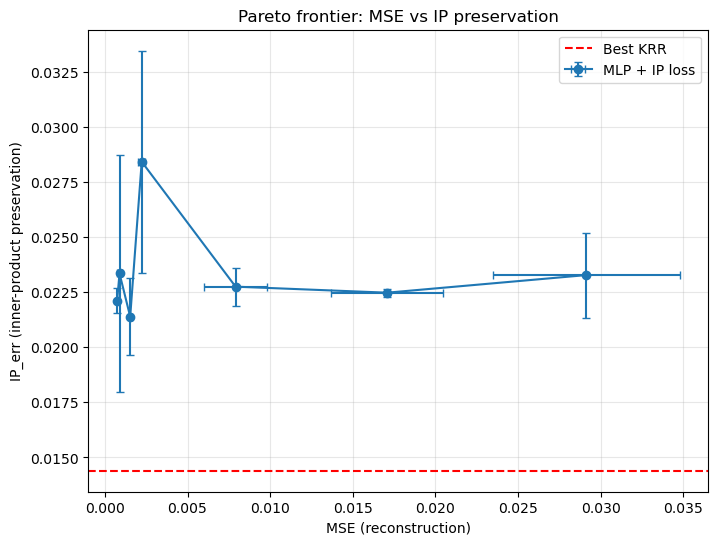
\includegraphics[width=0.7\textwidth]{pareto_frontier.png}
\caption{Pareto frontier of the MLP with inner-product loss, varying the
loss weight $w_{\text{IP}}$ from 0 to 100. Each point is the mean across
three random seeds. The red dashed line indicates the best KRR result
(IP\_err $= 0.0144$), which lies strictly below the MLP curve.}
\label{fig:pareto}
\end{figure}

\subsection{Rank ablation: every direction matters}

We extract the learned linear map $A \in \mathbb{R}^{n \times d}$ from the
MLP's outputs and compute its singular value decomposition. For $n = 4$,
the singular values are approximately $(5.5, 5.3, 1.3, 0.8)$ for one seed
and similar for others; two are large and two are small.

We then ask how much of the map's behavior depends on each singular
direction. For each rank $r \in \{1, 2, 3, 4\}$, we truncate $A$ to its
top-$r$ singular directions and re-evaluate IP\_err. The results are shown
in Figure~\ref{fig:rank}.

Truncation to rank 3 degrades IP\_err from $0.044$ to $0.111$
(a factor of $2.5$); rank 2 to $0.187$ (factor $4.2$); rank 1 to $0.262$
(factor $5.9$). The degradation is monotonic, with no plateau at any rank.

This result is counterintuitive given the singular value spectrum: one
might expect the small singular directions to be negligible, but they carry
essential geometric information. Any direction removed causes a
substantial drop in inner-product preservation.

\begin{figure}[t]
\centering
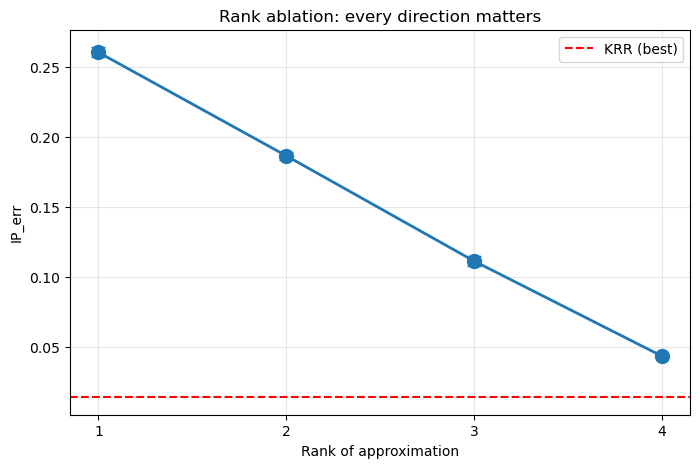
\includegraphics[width=0.6\textwidth]{rank_ablation.png}
\caption{Rank ablation of the learned linear map. Truncating the map to its
top-$r$ singular directions (for $r=1,\dots,4$) monotonically degrades
IP\_err, indicating that every direction is essential. The best KRR result
is shown as a horizontal dashed line for reference.}
\label{fig:rank}
\end{figure}

\subsection{Primary direction is target-driven}

We examine the primary direction of the learned map (the first right
singular vector of $A$, denoted $A_{\text{primary}}$) and compare it to
two candidate directions: the primary direction of the input latent space
$z_{\text{primary}}$ and the primary direction of the target angle space
$\theta_{\text{primary}}$.

The cosine similarity between $A_{\text{primary}}$ and $z_{\text{primary}}$
is $0.002$---essentially orthogonal. The cosine similarity between
$A_{\text{primary}}$ and $A^{\top} \theta_{\text{primary}}$, which lifts
$\theta_{\text{primary}}$ back into the input space via the learned map, is
$0.989$. The learned primary direction is therefore determined by the
geometry of the \emph{target} space, not by the input.

This is the key structural finding of the paper. It implies that the
mapping is not merely PCA-like projection of the input; it is a
target-driven transformation in which the network identifies which input
directions matter for the geometry of the output.

\begin{figure}[t]
\centering
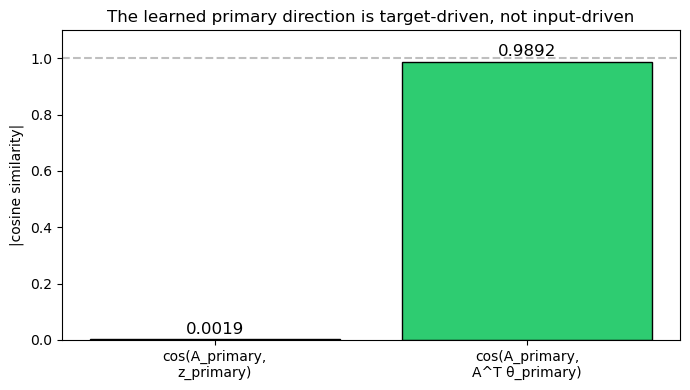
\includegraphics[width=0.55\textwidth]{primary_direction.png}
\caption{The learned primary direction is target-driven, not input-driven.
Cosine similarity with the input's principal direction is $0.002$;
similarity with the lifted target's principal direction is $0.989$.}
\label{fig:primary}
\end{figure}

\subsection{Subspace comparison: learned vs.\ PCA and seed-to-seed}

We compare the 4-dimensional subspace spanned by the rows of $A$ to the
4-dimensional PCA subspace used to construct the target. The principal
angles between these two subspaces are $(33.5^{\circ}, 68.0^{\circ},
88.6^{\circ}, 88.9^{\circ})$, with mean cosine $0.31$. The two subspaces
overlap only partially.

We also compare the learned subspace across the three random seeds. The
principal angles between seeds are $(1.5^{\circ}, 4.4^{\circ}, 40.2^{\circ},
78.4^{\circ})$ for seed 42 vs.\ 123, $(6.3^{\circ}, 8.2^{\circ},
48.2^{\circ}, 84.9^{\circ})$ for seed 42 vs.\ 7, and $(4.7^{\circ},
10.8^{\circ}, 38.2^{\circ}, 77.2^{\circ})$ for seed 123 vs.\ 7. All three
seeds agree on the first singular direction to within $6^{\circ}$; higher
directions diverge substantially.

Figure~\ref{fig:subspace} displays these principal angles as a heatmap. The
visualization makes two facts immediately clear: the learned subspace is
not the PCA subspace, and it is stable across seeds only in its primary
direction.

\begin{figure}[t]
\centering
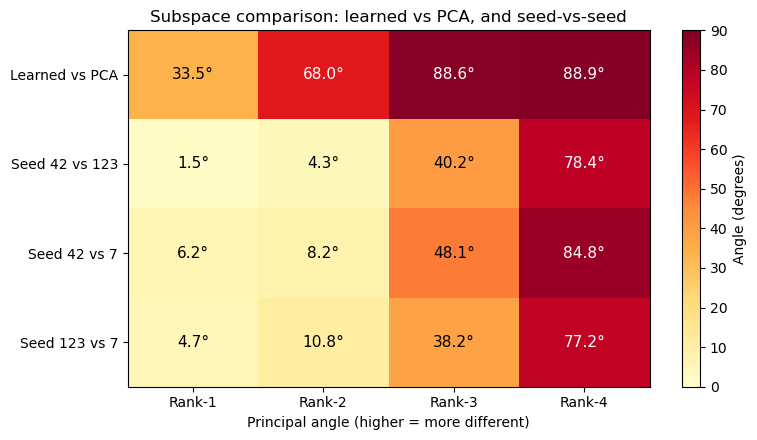
\includegraphics[width=0.75\textwidth]{subspace_heatmap.png}
\caption{Principal angles between the learned subspace and the PCA
subspace (top row) and between different random seeds (rows 2--4). All
seeds converge on the primary direction but diverge in higher ranks, and
none match the PCA basis used to construct the target.}
\label{fig:subspace}
\end{figure}

\subsection{Kernel ridge regression outperforms the MLP}

We train kernel ridge regression with an RBF kernel on the same 5{,}000
training pairs, sweeping $\alpha \in \{10^{-4}, 10^{-2}, 1\}$ and
$\gamma \in \{0.01, 0.1, 1\}$. The best configuration is
$\alpha = 10^{-4}$, $\gamma = 0.1$, achieving IP\_err $= 0.0144$ and
MSE $= 0.0013$.

For comparison, we sweep the MLP over 24 configurations varying the hidden
layer size, number of epochs, learning rate, and IP loss weight. The best
configuration is $h = 512$, 2{,}000 epochs, learning rate $10^{-3}$,
$w_{\text{IP}} = 1$, achieving IP\_err $= 0.0197$ and MSE $= 0.0015$.

The KRR result is better than the best MLP result by a factor of $1.37$ in
IP\_err. Both metrics favor the simpler method. Figure~\ref{fig:methods}
summarizes this comparison across all model classes.

\begin{figure}[t]
\centering
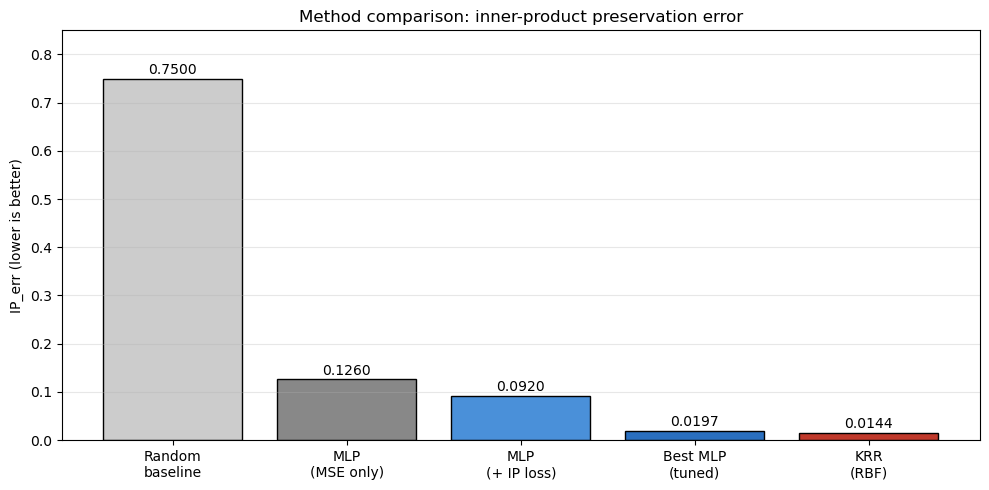
\includegraphics[width=0.75\textwidth]{method_comparison.png}
\caption{Inner-product preservation error across model classes. KRR
outperforms all neural configurations, including the tuned MLP.}
\label{fig:methods}
\end{figure}

\subsection{Stability across seeds}

For each qubit count $n \in \{2,3,4,5\}$ and each of three seeds, we train
a fresh MLP with inner-product loss. The mean IP\_err across seeds is
$0.065$ for $n=2$, $0.025$ for $n=3$, $0.032$ for $n=4$, and $0.047$ for
$n=5$. The standard deviation across seeds is largest for $n=2$ ($0.034$)
and smallest for $n=4$ ($0.0008$), indicating that the four-qubit result
is essentially deterministic.

The two-qubit case shows high variance, which we attribute to the small
dimension of the target space and the resulting flatness of the loss
landscape. The three- and four-qubit cases are stable, which supports the
robustness of the main findings.

\section{Discussion}
\label{sec:discussion}

Our results support four conclusions about structure-preserving latent-to-Hilbert
mappings in the controlled setting we studied.

First, the mapping is approximately linear in the latent vector. This
implies that linear methods---or methods with flexible but essentially
linear behavior, such as kernel ridge regression with an RBF kernel in the
small-$\gamma$ regime---are natural candidates. It also means that
practitioners working with similar problems should first try kernel methods
before investing in neural architecture design.

Second, the learned map requires all singular directions despite a highly
uneven singular value spectrum. This is a caution against rank-truncation
heuristics based on singular values alone: even small singular directions
can carry essential geometric information. The correct measure of
importance for structure-preserving maps is not the magnitude of the
singular value but the impact on the target metric.

Third, the learned primary direction is target-driven rather than
input-driven. The network does not simply project the input onto its
principal axes; it identifies the directions in the input space that matter
for the geometry of the target. This is a form of \emph{task-aware
dimensionality reduction}, and it may be a useful intuition for designing
more sophisticated structure-preserving architectures.

Fourth, in this setting, a classical kernel method outperforms the tuned
neural network. This does not mean that neural networks are never useful
for structure-preserving maps. Rather, it says that when the target mapping
is approximately linear and the scale is modest, a kernel method provides
a simpler and more accurate solution. The neural approach may become
preferable when the target is genuinely nonlinear---for example, when the
encoding includes entanglement between qubits or when the latent space is
larger and more complex.

We consider these implications preliminary but suggestive. They point
toward a research direction in which the geometry of the target space, and
the structure of the desired map, determine the appropriate model class,
rather than the reverse.

\section{Limitations and Future Work}
\label{sec:limitations}

The experiments reported in this paper are conducted at small scale. We use
5{,}000 MNIST images for training and a 1{,}000-image test set, with a
latent dimension of 8 and target Hilbert spaces of up to 5 qubits. It is
possible that results differ at larger scale.

Our target encoding is a product-state construction based on PCA of the
latent space. This choice is principled but specific; other encodings, in
particular those that include entanglement between qubits, may exhibit
different behavior. A natural extension is to test whether the observed
linearity and kernel-dominance effects persist when the target is an
entangled state.

We do not investigate the behavior of the mapping as a function of the
latent dimension or the autoencoder architecture. Future work could vary
these parameters to determine whether the primary direction remains
target-driven under a broader range of conditions.

Finally, our comparison between the MLP and KRR is at fixed hyperparameter
budgets. While we sweep 24 MLP configurations and 9 KRR configurations, it
is possible that more extensive tuning of either method would change the
relative ranking. The gap between KRR and the best MLP is $1.37$ in IP\_err,
which is substantial but not overwhelming.

\section{Conclusion}

We have studied whether a neural network can learn a structure-preserving
mapping from a compressed latent space to a Hilbert-space representation.
Our experiments show that the mapping is learnable, approximately linear,
and target-driven in its primary direction; that the learned map requires
all singular directions; and that kernel ridge regression outperforms a
tuned MLP in this setting. These results suggest that for
approximately-linear structure-preserving mappings, classical kernel
methods are a strong baseline and should be considered before more complex
neural approaches.

We hope that these findings contribute to a broader discussion of when
neural networks are the right tool for representation-learning tasks, and
when simpler methods suffice.

\bibliographystyle{plain}
\bibliography{refs}

\end{document}
